% Options for packages loaded elsewhere
\PassOptionsToPackage{unicode}{hyperref}
\PassOptionsToPackage{hyphens}{url}
%
\documentclass[
]{article}
\usepackage{amsmath,amssymb}
\usepackage{lmodern}
\usepackage{ifxetex,ifluatex}
\ifnum 0\ifxetex 1\fi\ifluatex 1\fi=0 % if pdftex
  \usepackage[T1]{fontenc}
  \usepackage[utf8]{inputenc}
  \usepackage{textcomp} % provide euro and other symbols
\else % if luatex or xetex
  \usepackage{unicode-math}
  \defaultfontfeatures{Scale=MatchLowercase}
  \defaultfontfeatures[\rmfamily]{Ligatures=TeX,Scale=1}
  \setmainfont[]{texgyrepagella-regular.otf}
  \setsansfont[]{Fira Sans}
\fi
% Use upquote if available, for straight quotes in verbatim environments
\IfFileExists{upquote.sty}{\usepackage{upquote}}{}
\IfFileExists{microtype.sty}{% use microtype if available
  \usepackage[]{microtype}
  \UseMicrotypeSet[protrusion]{basicmath} % disable protrusion for tt fonts
}{}
\makeatletter
\@ifundefined{KOMAClassName}{% if non-KOMA class
  \IfFileExists{parskip.sty}{%
    \usepackage{parskip}
  }{% else
    \setlength{\parindent}{0pt}
    \setlength{\parskip}{6pt plus 2pt minus 1pt}}
}{% if KOMA class
  \KOMAoptions{parskip=half}}
\makeatother
\usepackage{xcolor}
\IfFileExists{xurl.sty}{\usepackage{xurl}}{} % add URL line breaks if available
\IfFileExists{bookmark.sty}{\usepackage{bookmark}}{\usepackage{hyperref}}
\hypersetup{
  pdftitle={Supplementary Material},
  pdfauthor={Grant McDermott},
  hidelinks,
  pdfcreator={LaTeX via pandoc}}
\urlstyle{same} % disable monospaced font for URLs
\usepackage[margin=1in]{geometry}
\usepackage{graphicx}
\makeatletter
\def\maxwidth{\ifdim\Gin@nat@width>\linewidth\linewidth\else\Gin@nat@width\fi}
\def\maxheight{\ifdim\Gin@nat@height>\textheight\textheight\else\Gin@nat@height\fi}
\makeatother
% Scale images if necessary, so that they will not overflow the page
% margins by default, and it is still possible to overwrite the defaults
% using explicit options in \includegraphics[width, height, ...]{}
\setkeys{Gin}{width=\maxwidth,height=\maxheight,keepaspectratio}
% Set default figure placement to htbp
\makeatletter
\def\fps@figure{htbp}
\makeatother
\setlength{\emergencystretch}{3em} % prevent overfull lines
\providecommand{\tightlist}{%
  \setlength{\itemsep}{0pt}\setlength{\parskip}{0pt}}
\setcounter{secnumdepth}{-\maxdimen} % remove section numbering
\usepackage{fontspec}
\usepackage{float}
\usepackage{booktabs}
\usepackage{tabularx}
\usepackage{threeparttable}
\usepackage{dcolumn}
\DeclareMathOperator{\Var}{Var}
\newcolumntype{A}{D{.}{.}{2.3}}
\usepackage{sectsty} % Allows your to change titles style
\allsectionsfont{\sffamily} % Define the style of all titles
\usepackage{booktabs}
\usepackage{longtable}
\usepackage{array}
\usepackage{multirow}
\usepackage{wrapfig}
\usepackage{float}
\usepackage{colortbl}
\usepackage{pdflscape}
\usepackage{tabu}
\usepackage{threeparttable}
\usepackage{threeparttablex}
\usepackage[normalem]{ulem}
\usepackage{makecell}
\usepackage{xcolor}
\ifluatex
  \usepackage{selnolig}  % disable illegal ligatures
\fi
\usepackage[]{natbib}
\bibliographystyle{plainnat}

\title{Supplementary Material}
\usepackage{etoolbox}
\makeatletter
\providecommand{\subtitle}[1]{% add subtitle to \maketitle
  \apptocmd{\@title}{\par {\large #1 \par}}{}{}
}
\makeatother
\subtitle{Sceptic priors and climate consensus}
\author{Grant McDermott}
\date{}

\begin{document}
\maketitle

{
\setcounter{tocdepth}{2}
\tableofcontents
}
\newcommand{\beginsupplement}{%
    \setcounter{table}{0}
    \renewcommand{\thetable}{SM\arabic{table}}%
    \setcounter{figure}{0}
    \renewcommand{\thefigure}{SM\arabic{figure}}%
}
%
    \setcounter{table}{0}
    \renewcommand{\thetable}{SM\arabic{table}}%
    \setcounter{figure}{0}
    \renewcommand{\thefigure}{SM\arabic{figure}}%

\newpage

\hypertarget{sensitivity-analysis}{%
\section{Sensitivity analysis}\label{sensitivity-analysis}}

As noted in the main text, I consider a number of alternative
specifications to test the sensitivity of my findings. The following
section provides additional context and technical information for these
different sensitivity runs.

\textbf{Note:} Figs. \ref{fig:sens_cw14} -- \ref{fig:sens_co2} are
directly comparable to Fig. 1 in the main text and the same general
notes apply (dashed lines denote TCR priors, solid lines denote TCR
posteriors, etc.) In some cases, the x-axis has been truncated to
preserve this direct comparability, though the posterior distributions
extend beyond the -1 °C to 3 °C range. The caption of each figure
references against the key listed in Table 4 of the main text.

\hypertarget{alternative-gmst-series}{%
\subsection{Alternative GMST series}\label{alternative-gmst-series}}

HadCRUT4 is known to suffer from potential coverage biases due to
incomplete placement of \textit{in situ} thermometers. I therefore rerun
the analysis with two alternate reconstructions of GMST.
\cite{cowtan2014coverage}, hereafter CW14, correct for the gaps in the
HadCRUT4 dataset by using an interpolation algorithm based on the
``kriging'' method.\footnote{HadCRUT5 \citep{morice2020hadcrut5},
  released during the late revision stages of this manuscript, adopts a
  similar interpolation strategy to CW14. We would consequently expect
  this updated version of the HadCRUT temperature record to yield
  similar posterior results as CW14.} Similarly, the NASA Goddard
Institute for Space Studies uses an extrapolation algorithm to overcome
coverage bias in GISTEMP, its own GMST reconstruction. Running the
Bayesian regression model on these alternative series yields moderately
higher TCR values compared to HadCRUT4. Under a noninformative prior,
the posterior TCR means (and 95\% Bayesian credible intervals) are 1.6
°C (1.4--1.9 °C) for CW14 and 1.8 °C (1.5--2.0 °C) for GISTEMP. Given
that the explicit goal of this paper is to evaluate policy options from
the perspective of climate sceptics, I continue using the results from
the HadCRUT4 series as a default. Yet, it should be noted that this is a
conservative choice that may, at least marginally, understate the true
level of warming.

\begin{figure}[H]

{\centering 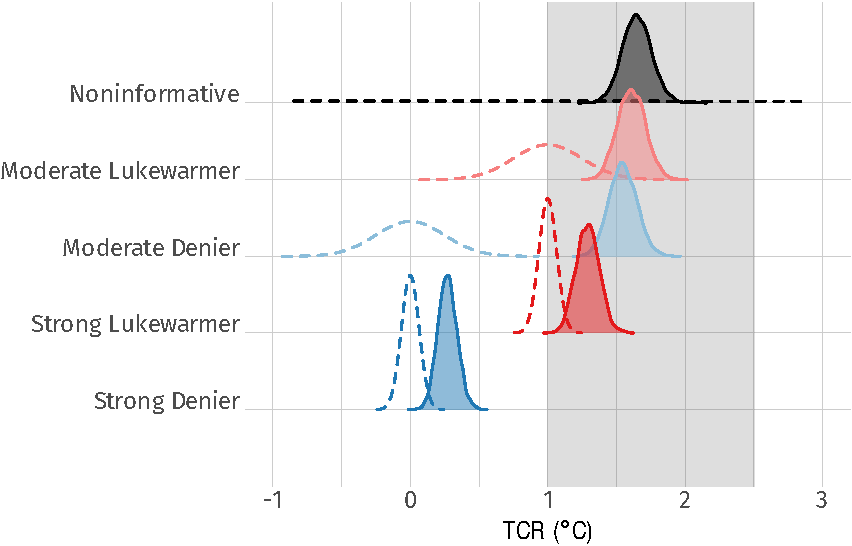
\includegraphics[width=1\linewidth]{/home/grant/Documents/Papers/Sceptic/sceptic-priors/figs/sens_cw14-1} 

}

\caption{TCR densities: "CW14" sensitivity run.}\label{fig:sens_cw14}
\end{figure}

\begin{figure}[H]

{\centering 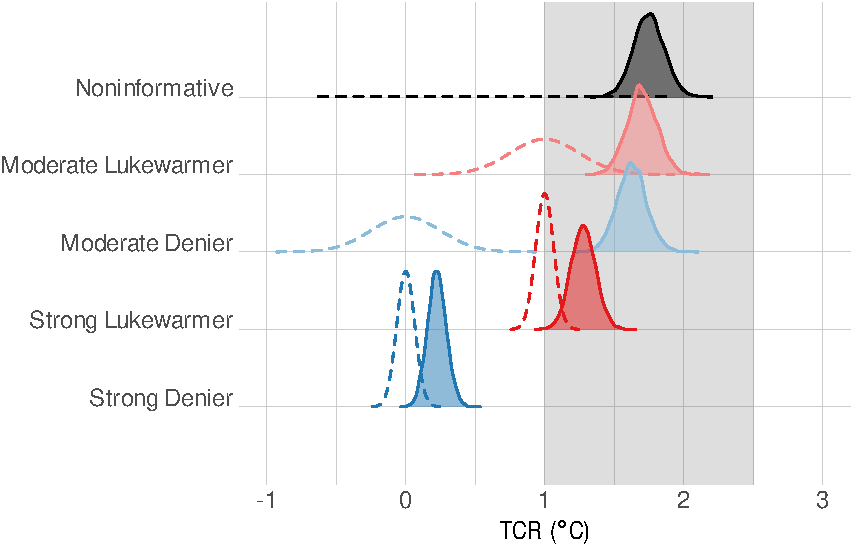
\includegraphics[width=1\linewidth]{/home/grant/Documents/Papers/Sceptic/sceptic-priors/figs/sens_gistemp-1} 

}

\caption{TCR densities: "GISTEMP" sensitivity run.}\label{fig:sens_gistemp}
\end{figure}

\newpage
\pagebreak

\hypertarget{measurement-error-in-gmst-data}{%
\subsection{Measurement error in GMST
data}\label{measurement-error-in-gmst-data}}

All three GMST reconstructions used in this study provide estimates of
measurement error. The Bayesian framework is ideally suited to
incorporate such knowledge, since the nested model structure allows us
to fully specify measurement error on the dependent variable within the
regression model itself. Doing so under the noninformative prior yields
TCR estimates of 1.6 °C (1.4--1.8 °C), which are effectively identical
to the comparable result in the main text. This is unsurprising once we
recall that measurement error on the dependent variable is absorbed by
the disturbance term of the regression model.\footnote{For example, see
  \cite[p. 326]{greene2007econometric}. To illustrate with a simple
  univariate case: The regression model can be written as
  \(y_t \sim \mathcal{N}(\beta X_t, \sigma^2 + \omega_t^2)\), where
  \(\sigma^2 = \mathop{\mathrm{Var}}(\epsilon)\) is the variance of the
  error term and \(\omega_t^2 = \mathop{\mathrm{Var}}(\nu_t)\) is the
  variance of the measurement error on \(y_t\). Together, \(\epsilon\)
  and \(\nu_t\) make up the overall disturbance of the regression.}
Since the Bayesian regression framework is primarily concerned with
total model uncertainty, specifying the relative contribution of such
measurement error to the overall disturbance doesn't meaningfully alter
the analysis --- though it may be useful for incorporating known sources
of heteroscedasticity.\footnote{See \cite{lewis2005edv} for a related
  discussion in a frequentist setting.} The primary regression results
already have GMST measurement error ``baked in'' to the estimation,
regardless of whether we define it explicitly or not.

\begin{figure}[H]

{\centering 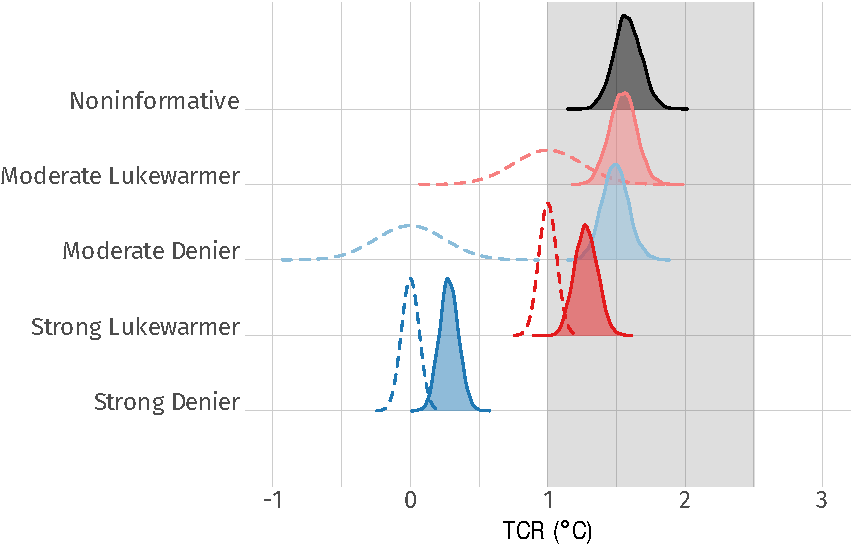
\includegraphics[width=1\linewidth]{/home/grant/Documents/Papers/Sceptic/sceptic-priors/figs/sens_hadcrut_me-1} 

}

\caption{TCR densities: "HadCRUT ME" sensitivity run.}\label{fig:sens_hadcrut_me}
\end{figure}

\newpage
\pagebreak

\hypertarget{measurement-error-in-forcings-data}{%
\subsection{Measurement error in forcings
data}\label{measurement-error-in-forcings-data}}

While measurement error in the dependent variable is already
(i.e.~implicitly) encapsulated by my Bayesian regression model, the same
cannot be said of any explanatory variables. In particular, uncertainty
about the radiative forcing data would need to be accounted for
explicitly in the modeling procedure. Fortunately, the Bayesian
framework offers a natural way to incorporate this type of uncertainty.
I conduct a Monte Carlo simulation using the 1,000-member ensemble of
forcing estimates from \cite{dessler2018ecs}; hereafter DF18.
Specifically, I run my Bayesian regression model on each member of the
DF18 ensemble separately --- 1,000 different regressions with each
taking their corresponding forcings as the true state of the world ---
before aggregating the posterior results into a single meta-distribution
at the end.\footnote{This probabilistic approach is the standard
  Bayesian solution to dealing with measurement error in explanatory
  variables. In contrast, deriving consistent regression estimators when
  there is measurement error in explanatory variables can be a much more
  complicated affair in frequentist settings
  \citep{greene2007econometric}.} The resulting posterior distributions
are wider, as expected due to the additional uncertainty. But the
noninformative TCR mean and 95\% credible interval of 1.4 °C (0.9--2.6
°C) are still well situated within the IPCC ``likely'' range.

\begin{figure}[H]

{\centering 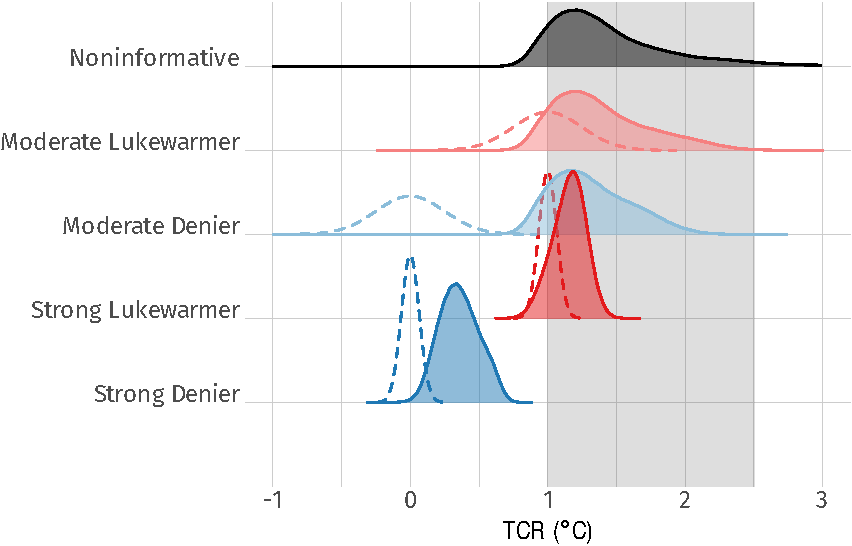
\includegraphics[width=1\linewidth]{/home/grant/Documents/Papers/Sceptic/sceptic-priors/figs/sens_df18-1} 

}

\caption{TCR densities: "DF18" sensitivity run.}\label{fig:sens_df18}
\end{figure}

\newpage
\pagebreak

\hypertarget{adjusted-forcing-efficacies}{%
\subsection{Adjusted forcing
efficacies}\label{adjusted-forcing-efficacies}}

The regression models in the main text implicitly assume that the
different physical drivers making up total radiative forcing have the
same per-unit effect on GMST. Forcing agents that yield a similar
radiative imbalance in Wm\(^{-2}\) are expected to result in similar
feedbacks and responses in GMST. However, recent research has suggested
that the warming efficacy of different forcing agents can, in fact, vary
with factors like geography. Aerosol emissions, for example, are
primarily concentrated in the mid-to-high latitudes of the Northern
Hemisphere. The disproportionately large land mass in this region causes
aerosol forcing to exhibit stronger feedback effects and an accelerated
temperature response than if it were uniformly distributed across the
globe \cite{shindell2014tcr}.

The implications of such forcing inhomogeneity on climate sensitivity
estimates are more fully explored by \cite{marvel2016implications},
hereafter MEA16. I adapt their results to construct an adjusted series
of total radiative forcing, where each forcing agent is pre-multiplied
by an appropriate efficacy coefficient (see Supplementary Material).
Specifically, I consider two approaches. The first takes MEA16's mean
efficacy estimates as given and ignores all modeling uncertainty in
their results. The second explicitly accounts for modeling uncertainty
in much the same way that was used to account for explanatory variable
measurement error above; i.e.~I conduct a Monte Carlo exercise that
repeatedly samples from the \emph{t} distributions underlying each
forcing efficacy estimate and then combines the posterior results from
many regressions into a single meta-distribution at the end. Consistent
with MEA16, both approaches lead to a pronounced increase in the
posterior TCR mean, with the Monte Carlo sampling approach further
yielding a much wider credible interval. However, MEA16 note that data
artefacts --- e.g.~small changes experienced by some forcing agents over
their study period --- automatically induce large uncertainties in the
associated efficacy estimates. Combined with the fact that MEA16 obtain
their results from a single climate model rather than a multi-model
ensemble, this means that the unusually wide credible intervals of the
latter Monte Carlo approach should be regarded with caution.

\begin{table}[ht] \centering 
    \caption{TCR efficacies used in ``MEA'' I and II sensitivity runs} 
    \label{tab:marvel} 
    \begin{threeparttable} 
        \begin{tabularx}{.75\textwidth}{@{\extracolsep{5pt}} Xcc}
            \toprule
            Forcing agent & Mean &   95\% C.I.   \\ 
            \midrule
            Aerosols      & 1.55 & (1.05, 2.05)  \\
            GHGs          & 1.17 & (1.07, 1.28)  \\
            Land use      & 3.82 & (-2.16, 9.80) \\
            Ozone         & 0.66 & (0.34, 0.98)  \\
            Solar         & 1.68 & (-1.27, 4.63)  \\
            Volcanic      & 0.61 & (0.33, 0.89)  \\ 
            \bottomrule
        \end{tabularx} 
        \begin{tablenotes}
            \footnotesize
            \item Notes: Adapted from Table S1 of \cite{marvel2016implications}. Confidence intervals on the sample means are constructed from a \textit{t} distribution with 4 degrees of freedom.
        \end{tablenotes}
    \end{threeparttable} 
\end{table}

\begin{figure}[H]

{\centering 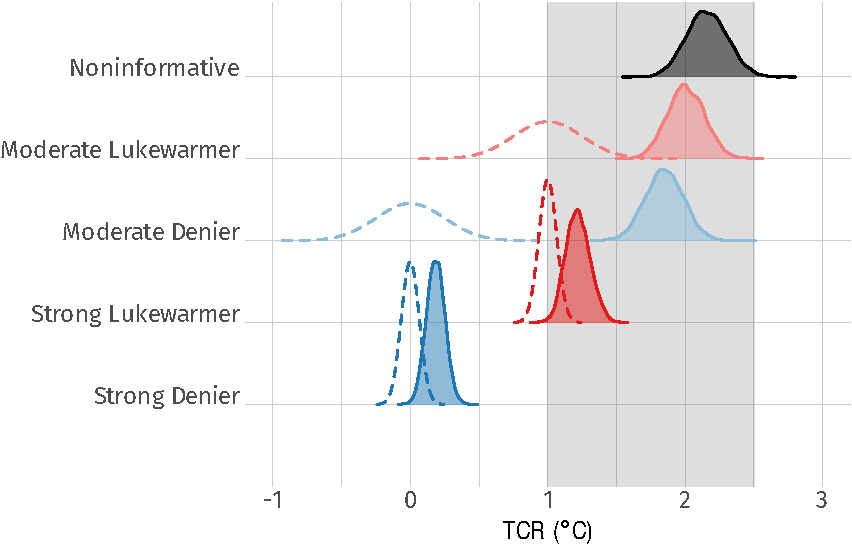
\includegraphics[width=1\linewidth]{/home/grant/Documents/Papers/Sceptic/sceptic-priors/figs/sens_mea_i-1} 

}

\caption{TCR densities: "MEA I" sensitivity run.}\label{fig:sens_mea_i}
\end{figure}

\begin{figure}[H]

{\centering 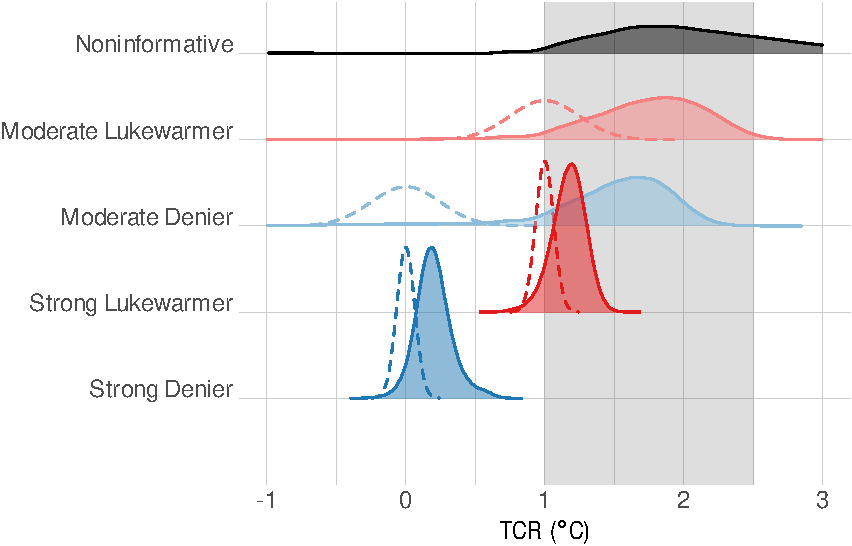
\includegraphics[width=1\linewidth]{/home/grant/Documents/Papers/Sceptic/sceptic-priors/figs/sens_mea_ii-1} 

}

\caption{TCR densities: "MEA II" sensitivity run.}\label{fig:sens_mea_ii}
\end{figure}

\newpage
\pagebreak

\hypertarget{separate-anthropogenic-forcings-co_2-from-other-forcings}{%
\subsection{\texorpdfstring{Separate anthropogenic forcings (CO\(_2\))
from other
forcings}{Separate anthropogenic forcings (CO\_2) from other forcings}}\label{separate-anthropogenic-forcings-co_2-from-other-forcings}}

As final sensitivity test, I relax the constraint that all sources of
radiative forcing have to be included in the regression model under the
same composite \(RF\) term. As described in the main text, this decision
was motivated by the fact that the forcing agents in my dataset are all
defined in Wm\(^{-2}\). Separating out individual forcings and then
placing different priors on them will likely cause the model to become
physically inconsistent.\footnote{For the anthropogenic forcings, the
  use of a composite term also avoids introducing severe
  multicollinearity into the econometric estimation.} Such admonishments
notwithstanding, I implement two version of this unphysical model. The
first separates out anthropogenic forcings (e.g.~GHGs) from natural
forcings (e.g.~solar radiation). The second separates out CO\(_2\)
forcing from all other sources. In each case, the subjective sceptic
priors are placed only on the isolated anthropogenic component. All
other variables take noninformative priors. Both sets of regressions
yield very similar results to the main, physically-correct
specification. If anything, isolating CO\(_2\) on its own yields a
higher posterior TCR for certain prior types. However, this latter
implementation should be treated with caution for reasons previously
described.

\begin{figure}[H]

{\centering 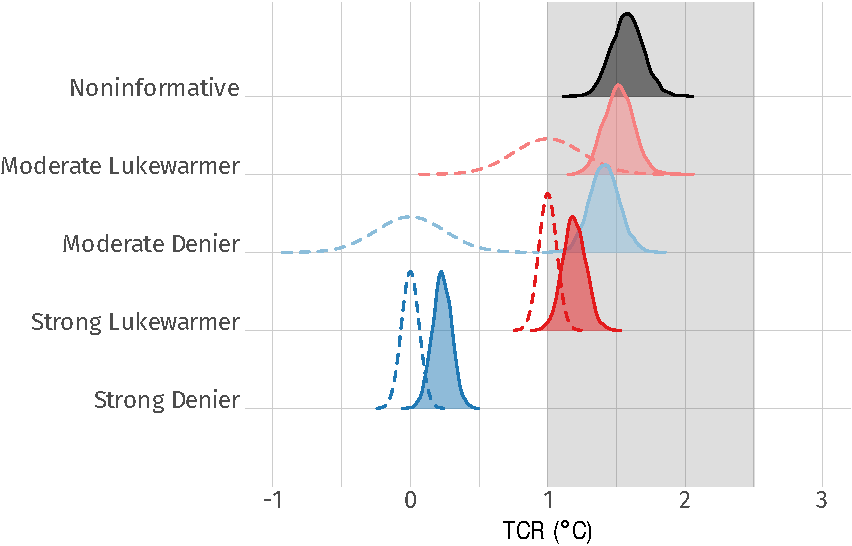
\includegraphics[width=1\linewidth]{/home/grant/Documents/Papers/Sceptic/sceptic-priors/figs/sens_anthro-1} 

}

\caption{TCR densities: "Anthro" sensitivity run.}\label{fig:sens_anthro}
\end{figure}

\begin{figure}[H]

{\centering 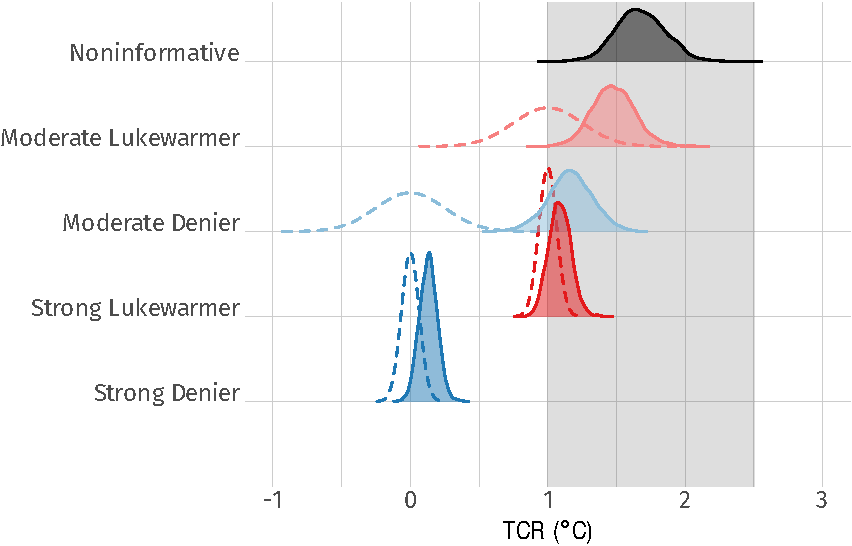
\includegraphics[width=1\linewidth]{/home/grant/Documents/Papers/Sceptic/sceptic-priors/figs/sens_co2-1} 

}

\caption{TCR densities: "CO2" sensitivity run.}\label{fig:sens_co2}
\end{figure}

\newpage
\pagebreak

\hypertarget{future-temperatures}{%
\section{Future temperatures}\label{future-temperatures}}

\begin{table}[h] \centering 
    \caption{Covariate vectors for 2100 predictions} 
    \begin{threeparttable} %%% added %%% 
        \begin{tabularx}{.75\textwidth}{@{\extracolsep{1pt}} X A A A A } 
            %\begin{tabularx}{\textwidth}{X c c c c} 
            %\hline\hline
            \toprule
            &\multicolumn{1}{c}{RCP 2.6}&\multicolumn{1}{c}{RCP 4.5}&\multicolumn{1}{c}{RCP 6.0}&\multicolumn{1}{c}{RCP 8.5}\\
            %&\multicolumn{1}{c}{\footnotesize420 ppmv CO$_2$}&\multicolumn{1}{c}{\footnotesize540 ppmv CO$_2$}&\multicolumn{1}{c}{\footnotesize670 ppmv CO$_2$}&\multicolumn{1}{c}{\footnotesize940 ppmv CO$_2$}\\
            %\hline
            %\\[-1.8ex] 
            \midrule
            $RF_{2100}$                                                                             & 2.626     & 4.281     & 5.522     & 8.340     \\ 
            \hspace{5 pt} \textit{CO$_2$ component} & \multicolumn{1}{c}{\textit{\hspace{1em}85\%}} &   \multicolumn{1}{c}{\textit{\hspace{1em}83\%}}   &   \multicolumn{1}{c}{\textit{\hspace{1em}86\%}}   &   \multicolumn{1}{c}{\textit{\hspace{1em}78\%}}   \\
            \hspace{5 pt} \textit{Solar component}      & \multicolumn{1}{c}{\textit{\hspace{1em} 7\%}} &   \multicolumn{1}{c}{\textit{\hspace{1em} 4\%}}   &   \multicolumn{1}{c}{\textit{\hspace{1em} 3\%}}   &   \multicolumn{1}{c}{\textit{\hspace{1em} 2\%}}   \\
            \\[-1.8ex] 
            $\overline{VOLC}$                                                                   & 0.017     & 0.017     & 0.017     & 0.017     \\
            \\[-1.8ex] 
            $\overline{SOI}$                                                                    &\text{-}0.079  &\text{-}0.079  &\text{-}0.079  &\text{-}0.079  \\
            \\[-1.8ex] 
            $\overline{AMO}$                                                                    &\text{-}0.002 &\text{-}0.002   &\text{-}0.002  &\text{-}0.002  \\
            %\hline\hline
            \bottomrule
        \end{tabularx}
        \begin{tablenotes}
            \footnotesize
            \item \textit{Notes:} Covariates are used to predict the global mean surface temperature anomaly in the year 2100. The Representative Concentration Pathways (RCPs) are a family of forcing scenarios developed for the IPCC \cite{van2011rcp}. Each RCP has a core component of atmospheric CO$_2$ concentrations, measured in parts per million volume (ppmv). With regard to the covariates in the regression model, total radiative forcing ($RF$) and volcanic aerosols ($VOLC$) are measured in Wm$^{-2}$. The Southern Oscillation Index ($SOI$) and Atlantic Multidecadal Oscilliation ($AMO$) are measured as scaled indices. Future values for $RF$ are taken from the RCP database. For the rest, historical mean values are used.
        \end{tablenotes}
    \end{threeparttable} 
    \label{tab:covariate}
\end{table}

\newpage
\pagebreak

\hypertarget{welfare-implications-and-the-social-cost-of-carbon}{%
\section{Welfare implications and the social cost of
carbon}\label{welfare-implications-and-the-social-cost-of-carbon}}

\begin{figure}[h]

{\centering 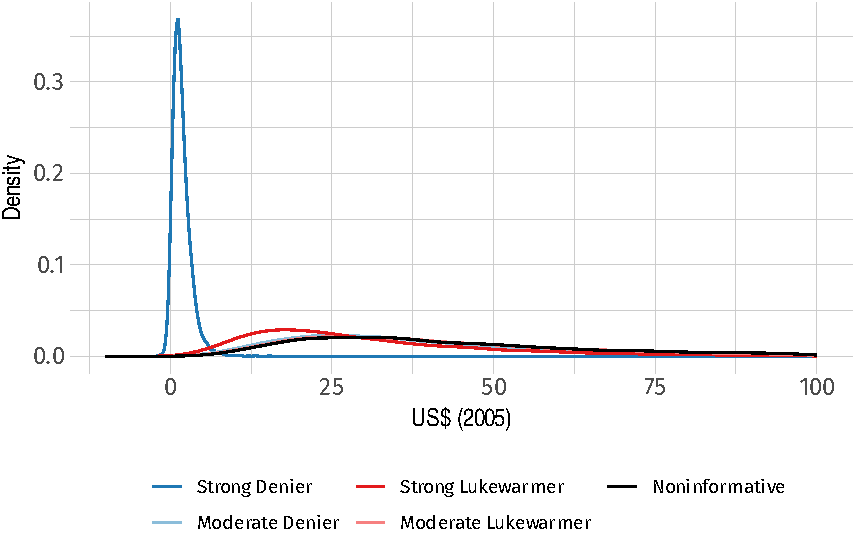
\includegraphics[width=1\linewidth]{/home/grant/Documents/Papers/Sceptic/sceptic-priors/figs/scc-fig-1} 

}

\caption{Social cost of carbon (US\$2020 per ton). SCC densities are generated by the MimiPAGE2009 model \citep{moore2018mimipage}, with the regression posterior TCR distributions for each prior type serving as key inputs. Model defaults are used for all other parameters. The x-axis is truncated at 100 to aid visual inspection; the uppermost tails of the distributions being well in excess of the range given here.}\label{fig:scc-fig}
\end{figure}

\newpage

  \bibliography{../sceptic/sceptic.bib}

\end{document}
